% Generated 2021-02-25 22:49:49 +0530
\subsection{Assets} \label{sec:Assets}


\block{Assets} \glspl{organize} the \block{Asset} types. \sect{Asset} provides the common semantic information for all the \block{Asset} types.

\begin{figure}[ht]
  \centering
    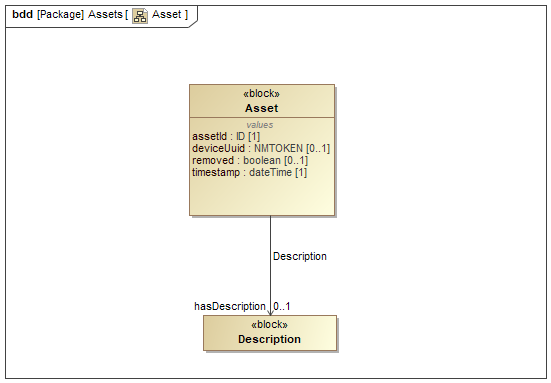
\includegraphics[width=1.0\textwidth]{figures/Asset.png}
  \caption{Asset Diagram}
  \label{fig:Asset Diagram}
\end{figure}

\FloatBarrier


Note: See \sect{Assets Schema Diagrams} for XML schema.


\subsubsection{Asset}
\label{sec:Asset}



\block{Asset} is an \gls{MTConnect Asset}. It is used in the manufacturing process, but is not permanently associated with a single piece of equipment. It can be removed from the piece of equipment without compromising its function, and can be associated with other pieces of equipment during its lifecycle.


\paragraph{Attributes of Asset}\mbox{}
\label{sec:Attributes of Asset}

\tbl{Attributes of Asset} lists the attributes of \texttt{Asset}.

\begin{table}[ht]
\centering 
  \caption{Attributes of Asset}
  \label{table:Attributes of Asset}
\tabulinesep=3pt
\begin{tabu} to 6in {|l|l|l|} \everyrow{\hline}
\hline
\rowfont\bfseries {Attribute} & {Type} & {Multiplicity} \\
\tabucline[1.5pt]{}

\property{assetId}[Asset] & \texttt{ID} & 1 \\
\property{deviceUuid}[Asset] & \texttt{NMTOKEN} & 0..1 \\
\property{removed}[Asset] & \texttt{boolean} & 0..1 \\
\property{timestamp}[Asset] & \texttt{dateTime} & 1 \\
\end{tabu}
\end{table}
\FloatBarrier

Descriptions for attributes of \block{Asset}:

\begin{itemize}

\item \property{assetId}[Asset] \newline The unique identifier for an \block{Asset}.

\item \property{deviceUuid}[Asset] \newline The piece of equipment's uuid that supplied the \block{Asset}'s data.

\item \property{removed}[Asset] \newline An indicator that the \block{Asset} has been removed from the piece of equipment.

\item \property{timestamp}[Asset] \newline The point in time the \block{Asset} data was last modified.
\end{itemize}


\paragraph{Elements of Asset}\mbox{}
\label{sec:Elements of Asset}

\tbl{Elements of Asset} lists the elements of \texttt{Asset}.

\begin{table}[ht]
\centering 
  \caption{Elements of Asset}
  \label{table:Elements of Asset}
\tabulinesep=3pt
\begin{tabu} to 6in {|l|l|} \everyrow{\hline}
\hline
\rowfont\bfseries {Element} & {Multiplicity} \\
\tabucline[1.5pt]{}
\texttt{Description} & 0..1 \\
\end{tabu}
\end{table}
\FloatBarrier


Descriptions for elements of \block{Asset}:

\begin{itemize}

\item \block{Description} \newline The descriptive content. This can contain configuration information and manufacturer specific details.
\end{itemize}


